\chapter{Organização funcional de um mamífero}\label{ch:b1:mammal-organization}

Abra um coelho na mesa de dissecção e a primeira impressão é de ordem.
Uma lâmina muscular, o \omterm{def:b1:mammal-organization:bodyplan}{diafragma}, divide o tronco em um tórax que abriga
o coração e dois pulmões e um abdome que abriga todo o resto: um fígado
do tamanho de um punho, um estômago, quatro metros de intestino
terminando num ceco tão grande quanto o estômago, dois rins encostados
na parede posterior. Cada \omterm{def:b1:mammal-organization:organ}{órgão} tem um lugar, uma irrigação e uma
tarefa; nenhum deles trabalha sozinho. Este capítulo descreve como o
mamífero é construído como um todo em funcionamento: o \omterm{def:b1:mammal-organization:bodyplan}{plano de
organização} dele, os sistemas em que os \omterm{def:b1:mammal-organization:organ}{órgãos} se agrupam, os
compartimentos líquidos em que as células vivem, as \omterm{prop:b1:organism-environment:surfaces}{superfícies de troca}
pelas quais ele encontra o exterior, e o balanço térmico que o mantém a
\qty{39}{\celsius} num campo de janeiro.

\section{O plano de organização de um mamífero}

\begin{definition}[Plano de organização]\label{def:b1:mammal-organization:bodyplan}
O \emph{plano de organização}\index{plano de organização} de um animal é
a disposição dos eixos, das cavidades e dos \omterm{def:b1:mammal-organization:organ}{órgãos} dele que é comum a
todos os membros do grupo. O plano de organização dos mamíferos é o de
um vertebrado: simetria bilateral com uma extremidade cefálica que leva
o encéfalo e os principais \omterm{def:b1:mammal-organization:organ}{órgãos} dos sentidos
(\emph{cefalização}\index{cefalização}), um eixo dorsal de vértebras que
envolve a medula espinal, quatro membros e uma cavidade corporal ventral
--- o \emph{celoma}\index{celoma} --- que contém as vísceras. O que é
especificamente mamífero: o celoma é dividido pelo
\emph{diafragma}\index{diafragma} muscular em uma cavidade torácica
(coração, pulmões) e uma cavidade abdominal (\omterm{def:b1:mammal-organization:organ}{órgãos} digestórios, rins,
gônadas); o corpo é coberto de pelos; os filhotes são alimentados com
leite; a temperatura é regulada.
\end{definition}

\begin{omfigure}
\begin{tikzpicture}
  \node[anchor=south west, inner sep=0] (img) at (0,0)
    {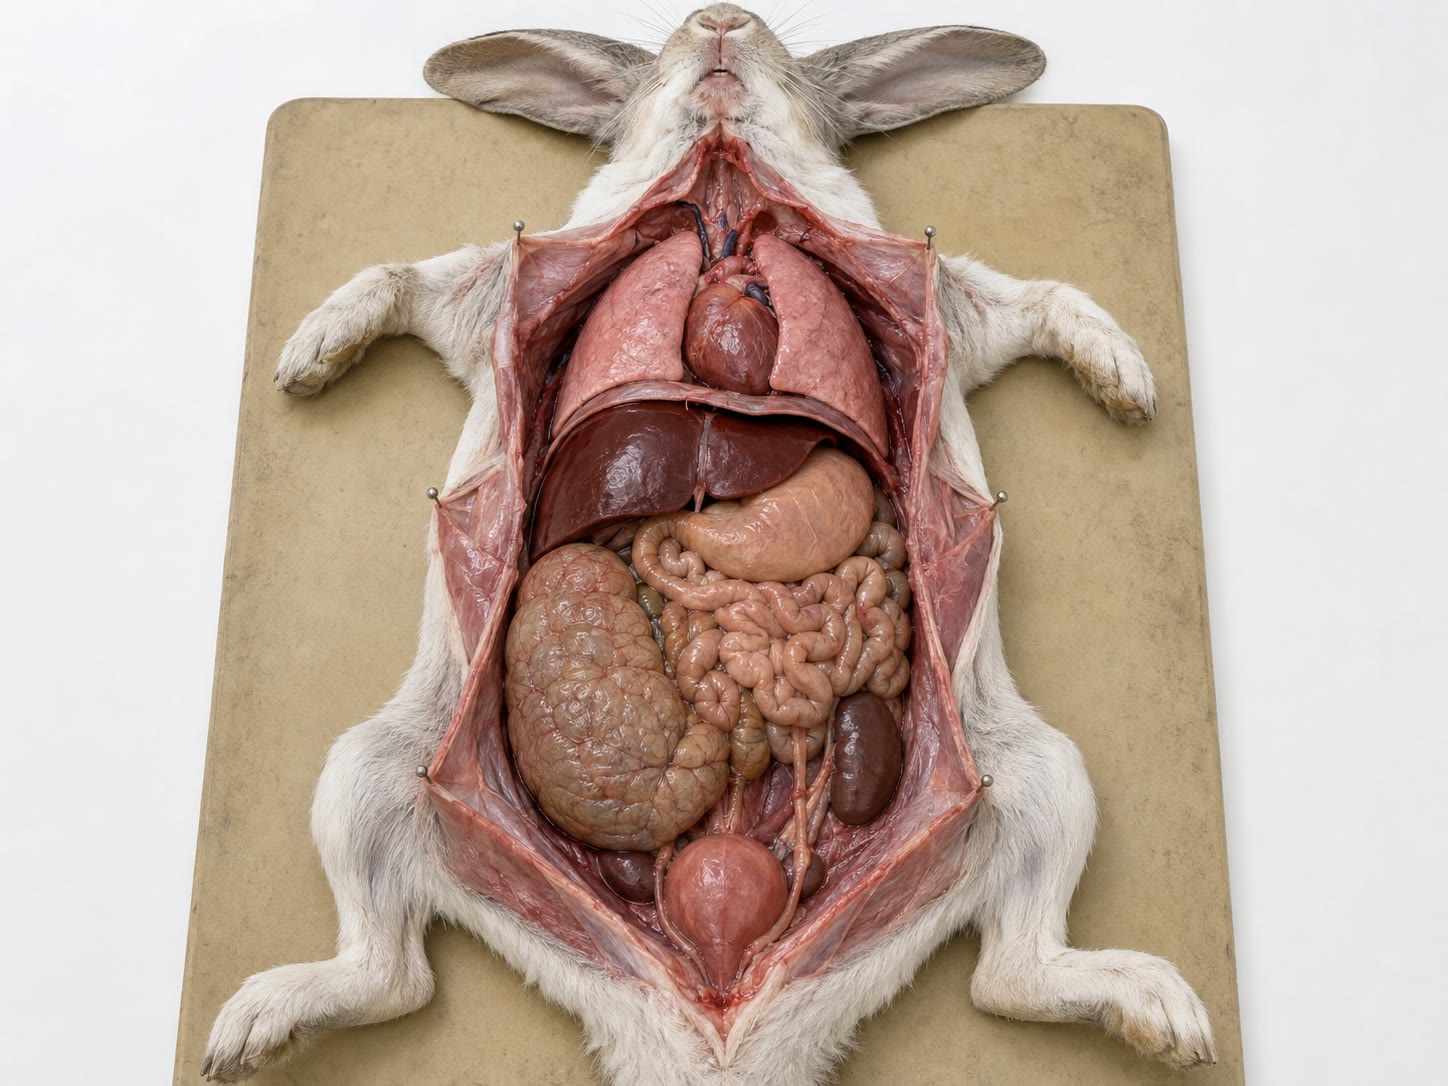
\includegraphics[width=0.6\linewidth]{images/book3/ai/fig-rabbit-dissection.jpg}};
  \begin{scope}[x={(img.south east)}, y={(img.north west)},
      every node/.style={font=\small}]
    \draw[omDef, thick] (0.44,0.72) -- (-0.02,0.90) node[left] {pulmões};
    \draw[omDef, thick] (0.50,0.68) -- (1.02,0.88) node[right] {coração};
    \draw[omDef, thick] (0.53,0.61) -- (1.02,0.70) node[right] {diafragma};
    \draw[omDef, thick] (0.44,0.55) -- (-0.02,0.62) node[left] {fígado};
    \draw[omDef, thick] (0.56,0.52) -- (1.02,0.54) node[right] {estômago};
    \draw[omDef, thick] (0.52,0.42) -- (1.02,0.40) node[right] {intestino delgado};
    \draw[omDef, thick] (0.42,0.36) -- (-0.02,0.36) node[left] {ceco};
    \draw[omDef, thick] (0.60,0.30) -- (1.02,0.24) node[right] {rim};
    \draw[omDef, thick] (0.51,0.17) -- (-0.02,0.10) node[left] {bexiga};
  \end{scope}
\end{tikzpicture}

{\small Um coelho aberto pelo lado ventral. O \omterm{def:b1:mammal-organization:bodyplan}{diafragma} separa a
cavidade torácica (pulmões, coração) da cavidade abdominal (fígado,
estômago, intestino, ceco, rins, bexiga). Cada \omterm{def:b1:mammal-organization:organ}{órgão} fica num lugar
fixo, envolvido por uma membrana e irrigado pelos próprios vasos.}
\end{omfigure}

\begin{definition}[Órgão, sistema de órgãos]\label{def:b1:mammal-organization:organ}
Um \emph{órgão}\index{órgão} é uma estrutura feita de vários tecidos
(\cref{ch:b1:body-plans-tissues}) dispostos para desempenhar uma função
definida: o coração bombeia, o pulmão troca gases, o rim filtra. Um
\emph{sistema de órgãos}\index{sistema de órgãos} é um conjunto de
órgãos que cooperam em uma função ampla: o sistema digestório vai da
boca ao ânus, com o fígado e o pâncreas anexos; o sistema circulatório é
o coração e os vasos; o sistema excretor, os rins e as vias urinárias.
\end{definition}

\section{Os sistemas de órgãos e as funções que eles servem}

\begin{proposition}[Três grupos de funções]\label{prop:b1:mammal-organization:functions}
Os \omterm{def:b1:mammal-organization:organ}{sistemas de órgãos} de um mamífero servem a três grupos de funções:
\begin{itemize}
  \item \emph{nutrição}\index{função de nutrição}: captar e distribuir
        matéria e energia e eliminar dejetos --- os sistemas digestório,
        respiratório, circulatório e excretor;
  \item \emph{relação}\index{função de relação}: perceber o ambiente e
        agir sobre ele --- os \omterm{def:b1:mammal-organization:organ}{órgãos} dos sentidos, o sistema nervoso, as
        glândulas endócrinas, o esqueleto e os músculos;
  \item \emph{reprodução}\index{função de reprodução}: produzir
        descendentes --- as gônadas, o trato genital e, nos mamíferos,
        as glândulas mamárias.
\end{itemize}
Nenhum sistema trabalha sozinho: todo \omterm{def:b1:mammal-organization:organ}{órgão} depende do sangue para ser
abastecido, dos sistemas nervoso e endócrino para ser coordenado, e do
esqueleto e da pele para ser protegido.
\end{proposition}

\begin{omfigure}
\begin{tikzpicture}[font=\footnotesize, >=Stealth, line cap=round,
  sys/.style={draw, thick, rounded corners=3pt, minimum height=7mm, minimum width=24mm, align=center, fill=white},
  lab/.style={font=\scriptsize, above},
  grp/.style={font=\small\bfseries, anchor=west}]
  \node[grp, omProp] at (0,4.6) {Nutrição};
  \node[sys, fill=omProp!12] (dig) at (1.3,3.8) {digestório};
  \node[sys, fill=omProp!12] (res) at (1.3,2.9) {respiratório};
  \node[sys, fill=omProp!12] (exc) at (1.3,2.0) {excretor};
  \node[grp, omExo] at (0,1.1) {Reprodução};
  \node[sys, fill=omExo!12] (gen) at (1.3,0.3) {genital};
  \node[sys, fill=omThm!12, minimum height=30mm] (cir) at (5.9,2.6) {circulatório\\ (sangue, linfa)};
  \node[grp, omDef] at (8.6,4.6) {Relação};
  \node[sys, fill=omDef!12, minimum width=30mm] (ner) at (10.3,3.8) {nervoso, sentidos};
  \node[sys, fill=omDef!12, minimum width=30mm] (end) at (10.3,2.9) {endócrino};
  \node[sys, fill=omDef!12, minimum width=30mm] (mus) at (10.3,2.0) {esqueleto, músculos};
  \node[sys, fill=omDef!12, minimum width=30mm] (ski) at (10.3,1.1) {pele};
  \draw[<->, thick] (dig.east) -- (cir.west |- dig.east) node[lab, midway] {nutrientes};
  \draw[<->, thick] (res.east) -- (cir.west |- res.east) node[lab, midway] {$\mathrm{O_2}$, $\mathrm{CO_2}$};
  \draw[<->, thick] (exc.east) -- (cir.west |- exc.east) node[lab, midway] {dejetos};
  \draw[<->, thick] (gen.east) -- ++(1.6,0) |- (cir.south west);
  \draw[<->, thick] (cir.east |- ner.west) -- (ner.west);
  \draw[<->, thick] (cir.east |- end.west) -- (end.west) node[lab, midway] {hormônios};
  \draw[<->, thick] (cir.east |- mus.west) -- (mus.west);
  \draw[<->, thick] (cir.south east) -| ++(0.5,0) |- (ski.west);
\end{tikzpicture}

{\small Os \omterm{def:b1:mammal-organization:organ}{sistemas de órgãos} de um mamífero agrupados por função. A
circulação é o eixo central: todo sistema troca com o sangue, e o sangue
leva a todos os outros o que um sistema capta.}
\end{omfigure}

\begin{example}[Uma bocada de capim]\label{ex:b1:mammal-organization:mouthful}
O capim do coelho é cortado pelos incisivos e moído pelos molares
(esqueleto e músculos), degustado e cheirado (sentidos), engolido e
digerido no estômago e no intestino delgado; os açúcares e os
aminoácidos dele atravessam a parede intestinal para o sangue e chegam
ao fígado, que os armazena ou os libera sob controle hormonal
(endócrino); a celulose dele é fermentada por bactérias no ceco; o
oxigênio para queimar os açúcares vem pelos pulmões, o dióxido de
carbono sai pelo mesmo caminho, a ureia dos aminoácidos sai pelos rins,
e o calor de todo o processo sai pela pele. Sete sistemas para uma
bocada.
\end{example}

\section{Os compartimentos do corpo}

\begin{definition}[Compartimentos líquidos]\label{def:b1:mammal-organization:compartments}
A água representa cerca de \qty{60}{\%} da massa de um mamífero. Dois
terços dela são \emph{líquido intracelular}\index{líquido intracelular},
dentro das células; um terço é
\emph{líquido extracelular}\index{líquido extracelular}, o \omterm{def:b1:organism-environment:milieu}{meio interno}
do \cref{ch:b1:organism-environment}, ele mesmo dividido no
\emph{líquido intersticial}\index{líquido intersticial} que banha as
células (três quartos dele) e no \emph{plasma sanguíneo}\index{plasma}
dentro dos vasos (um quarto). A \emph{linfa}\index{linfa} é líquido
intersticial recolhido pelos vasos linfáticos e devolvido ao sangue. Os
dois líquidos extracelulares têm composição quase idêntica --- o plasma
difere pelas proteínas dele, que não atravessam a parede capilar --- e
os dois diferem nitidamente do líquido intracelular.
\end{definition}

\begin{omfigure}
\begin{tikzpicture}[font=\small, line cap=round]
  \draw[thick, fill=gray!8, rounded corners=6pt] (0,0) rectangle (11.6,4.6);
  \node[anchor=north west, font=\small\bfseries] at (0.15,4.55) {água corporal total: \qty{42}{L} (\qty{60}{\%} de \qty{70}{kg})};
  \draw[thick, fill=omDef!14, rounded corners=5pt] (0.3,0.3) rectangle (6.4,3.8);
  \node[anchor=north west, align=left] at (0.4,3.7) {\textbf{líquido intracelular}: \qty{28}{L}\\ muito $\mathrm{K^+}$ (\qty{140}{mmol/L}),\\ fosfato, proteínas;\\ pouco $\mathrm{Na^+}$ (\qty{10}{mmol/L})};
  \draw[thick, fill=omProp!14, rounded corners=5pt] (6.7,0.3) rectangle (11.3,3.8);
  \node[anchor=north west, align=left] at (6.8,3.7) {\textbf{líquido extracelular}: \qty{14}{L}\\ muito $\mathrm{Na^+}$ (\qty{140}{mmol/L}),\\ $\mathrm{Cl^-}$, $\mathrm{HCO_3^-}$};
  \draw[thick, fill=omProp!30, rounded corners=4pt] (6.9,0.45) rectangle (9.2,1.55);
  \node[align=center, font=\footnotesize] at (8.05,1.0) {intersticial\\ \qty{11}{L}};
  \draw[thick, fill=omThm!30, rounded corners=4pt] (9.4,0.45) rectangle (11.1,1.55);
  \node[align=center, font=\footnotesize] at (10.25,1.0) {plasma\\ \qty{3}{L}};
\end{tikzpicture}

{\small Os compartimentos líquidos de um ser humano de \qty{70}{kg}.
Dois terços da água estão dentro das células; o terço extracelular,
repartido entre o \omterm{def:b1:mammal-organization:compartments}{líquido intersticial} e o plasma, é o \omterm{def:b1:organism-environment:milieu}{meio interno}. O
sódio domina do lado de fora e o potássio do lado de dentro --- uma
diferença que toda célula gasta energia para manter
(\cref{ch:b1:membranes-transport}).}
\end{omfigure}

\begin{method}[Medir um compartimento por diluição]\label{met:b1:mammal-organization:dilution}
\begin{enumerate}
  \item Escolha um marcador que se distribua no compartimento e em
        nenhum outro: um corante ligado às proteínas do plasma (azul de
        Evans) para o plasma; a inulina, um açúcar que sai dos vasos mas
        não entra nas células, para o \omterm{def:b1:mammal-organization:compartments}{líquido extracelular}; a água
        pesada para a água corporal total.
  \item Injete uma quantidade conhecida $m$ e espere a mistura (minutos
        para o plasma, horas para a água total).
  \item Meça a concentração $c$ em uma amostra de plasma, corrigindo
        qualquer perda (urina, metabolismo) durante a espera.
  \item O volume é $V = m/c$. O volume intracelular é a água total menos
        a extracelular; o volume intersticial é o extracelular menos o
        plasma. O volume de sangue é o volume de plasma dividido pela
        fração de plasma no sangue ($1 - $ hematócrito).
\end{enumerate}
\end{method}

\begin{example}[Um volume de plasma]\label{ex:b1:mammal-organization:evansblue}
\qty{50}{mg} de azul de Evans injetados em um homem de \qty{70}{kg} dão,
dez minutos depois, uma concentração plasmática de \qty{16.7}{mg/L}:
$V = 50/16.7 = \qty{3.0}{L}$ de plasma. Com um hematócrito de
\qty{45}{\%}, o volume de sangue é $3.0/0.55 = \qty{5.5}{L}$ ---
\qty{8}{\%} da massa corporal, uma proporção que vale do camundongo à
baleia.
\end{example}

\section{Superfícies de troca e circulação}

\begin{proposition}[Toda superfície de troca está acoplada ao sangue]\label{prop:b1:mammal-organization:surfaces}
Um mamífero troca com o exterior por quatro superfícies, cada uma
dobrada dentro do corpo e cada uma irrigada por uma rede capilar densa:
a mucosa intestinal (\qty{30}{m^2} num ser humano) para os nutrientes e
a água, a superfície alveolar dos pulmões (\qty{100}{m^2}) para o
oxigênio e o dióxido de carbono, a superfície filtrante dos rins (um
milhão de glomérulos, que filtram \qty{180}{L} de plasma por dia) para
os dejetos e para a regulação do \omterm{def:b1:organism-environment:milieu}{meio interno}, e a pele (\qty{2}{m^2})
para o calor e um pouco de água. A circulação as liga: o sangue que sai
de uma superfície chega à seguinte em menos de um minuto, de modo que o
que entra pelo intestino é oxidado com o oxigênio do pulmão e o dejeto
resultante sai pelo rim.
\end{proposition}

\begin{omfigure}
\begin{tikzpicture}[font=\small, >=Stealth, line cap=round,
  org/.style={draw, thick, rounded corners=4pt, minimum height=8mm, minimum width=22mm, align=center, fill=white}]
  \node[org, fill=omDef!12] (lung) at (0,3.2) {pulmões\\ \qty{100}{m^2}};
  \node[org, fill=omThm!15, minimum width=26mm, minimum height=12mm] (heart) at (0,0) {coração\\ direito $\mid$ esquerdo};
  \node[org, fill=omProp!12] (gut) at (5.2,1.6) {intestino\\ \qty{30}{m^2}};
  \node[org, fill=omProp!12] (liver) at (5.2,0.0) {fígado};
  \node[org, fill=omProp!12] (kid) at (5.2,-1.6) {rins\\ \qty{180}{L/d}};
  \node[org, fill=omExo!12] (mus) at (5.2,3.2) {músculos, pele,\\ encéfalo, outros};
  % pulmonary loop
  \draw[->, very thick, omDef] (heart.north west) ++(-0.2,0) |- (lung.west) node[pos=0.25, left, font=\footnotesize, align=right] {circuito\\ pulmonar};
  \draw[->, very thick, omThm] (lung.east) -| ($(heart.north east)+(0.2,0)$);
  % systemic loop: left heart -> organs (parallel) -> right heart
  \draw[very thick, omThm] (heart.east) -- ++(1.2,0) coordinate (a);
  \draw[->, very thick, omThm] (a) |- (mus.west);
  \draw[->, very thick, omThm] (a) |- (gut.west);
  \draw[->, very thick, omThm] (a) |- (kid.west);
  \draw[->, very thick, omThm] (a) -- (liver.west);
  \draw[->, very thick, omDef] (gut.south) -- (liver.north) node[midway, right, font=\footnotesize] {veia porta};
  \coordinate (b) at (8.0,0.8);
  \draw[very thick, omDef] (mus.east) -| (b);
  \draw[very thick, omDef] (liver.east) -| (b);
  \draw[very thick, omDef] (kid.east) -| (b);
  \draw[->, very thick, omDef] (b) |- ++(0,-3.2) -| (heart.south) node[pos=0.25, below, font=\footnotesize] {circuito sistêmico: veias};
\end{tikzpicture}

{\small A dupla circulação de um mamífero. O coração direito envia
sangue pobre em oxigênio (azul) pelos pulmões; o coração esquerdo envia
sangue oxigenado (vermelho) pelos \omterm{def:b1:mammal-organization:organ}{órgãos}, dispostos em paralelo, de modo
que cada um recebe sangue arterial fresco. O sangue vindo do intestino
passa pelo fígado antes de voltar ao coração.}
\end{omfigure}

\begin{omfigure}
\begin{tikzpicture}
\begin{axis}[
  xbar, bar width=8pt,
  width=0.82\linewidth, height=6.2cm,
  axis x line=bottom, axis y line=left,
  xmin=0, xmax=1.8, xlabel={fluxo sanguíneo em repouso (\unit{L/min})},
  xlabel style={font=\small, at={(axis description cs:0.5,-0.13)}, anchor=north},
  symbolic y coords={músculo cardíaco, pele, encéfalo, músculo esquelético, rins, fígado e intestino},
  ytick=data, tick label style={font=\small},
  enlarge y limits=0.12, xtick={0,0.5,1.0,1.5},
  nodes near coords, nodes near coords style={font=\scriptsize, anchor=west},
]
\addplot[fill=omThm!45, draw=omThm] coordinates
  {(0.25,músculo cardíaco) (0.4,pele) (0.75,encéfalo) (1.0,músculo esquelético) (1.1,rins) (1.35,fígado e intestino)};
\end{axis}
\end{tikzpicture}

{\small Como um débito cardíaco humano de \qty{5}{L/min} em repouso é
repartido entre os \omterm{def:b1:mammal-organization:organ}{órgãos}. Os rins, \qty{0.5}{\%} da massa corporal,
recebem um quinto do sangue --- o preço de filtrar todo o plasma
sessenta vezes por dia. Durante o exercício a parcela dos músculos sobe
dez vezes e a do intestino cai.}
\end{omfigure}

\begin{example}[O tempo de circulação]\label{ex:b1:mammal-organization:circtime}
Com \qty{5.5}{L} de sangue e um débito cardíaco de \qty{5}{L/min}, uma
gota de sangue completa o duplo circuito em cerca de um minuto em
repouso, e em um quarto disso durante exercício intenso, quando o débito
chega a \qty{20}{L/min}. O débito cardíaco escala como $M^{3/4}$
(\cref{thm:b1:organism-environment:kleiber}): o de um coelho de
\qty{2}{kg} é de cerca de \qty{0.35}{L/min} para \qty{160}{mL} de
sangue --- o mesmo tempo de circulação a menos de um fator dois, com uma
frequência cardíaca de \qty{200}{} batimentos por minuto.
\end{example}

\section{Endotermia e balanço térmico}

\begin{proposition}[O balanço de calor]\label{prop:b1:mammal-organization:heatbudget}
\index{balanço de calor}
Um mamífero em temperatura estacionária satisfaz
\[
M - W = R + C + K + E ,
\]
em que $M$ é a produção metabólica de calor, $W$ o trabalho mecânico
realizado sobre o exterior, e o lado direito são as perdas por radiação
$R$, convecção para o ar $C$, condução para o solo $K$ e evaporação $E$
(pelos pulmões e pelo suor ou pelo ofego). As três primeiras perdas são
proporcionais a $T_b - T_a$ e são governadas pelo isolamento da pelagem
e pelo fluxo de sangue para a pele; a evaporação é a única via que
funciona quando o ar está mais quente que o corpo. Quando a equação não
é satisfeita, a temperatura corporal deriva a uma taxa fixada pelo
desequilíbrio e pela capacidade térmica do corpo (cerca de
\qty{3.5}{kJ.kg^{-1}.K^{-1}}).
\end{proposition}
\begin{proof}
Conservação da energia para o corpo ao longo de um período em que a
temperatura dele não muda: a energia química liberada ($M$) sai como
trabalho ou como calor pelos quatro canais físicos. A proporcionalidade
de $R$, $C$ e $K$ à diferença de temperatura é a lei do resfriamento de
Newton (\cref{ch:b1:organism-environment}); a independência de $E$ em
relação a essa diferença decorre de a evaporação ser impulsionada pelo
gradiente de umidade, e não pelo de temperatura.
\end{proof}

\begin{omfigure}
\begin{tikzpicture}[font=\small, >=Stealth, line cap=round]
  \draw[very thick, fill=omThm!8, rounded corners=16pt] (0,0) rectangle (5.0,3.0);
  \node[align=center] at (2.5,1.5) {centro do corpo a \qty{39}{\celsius}\\ produção de calor $M$\\ (basal, tremor, atividade)};
  \draw[->, very thick, omThm] (5.0,2.5) -- (6.6,2.5) node[right, align=left] {$R$: radiação para\\ as paredes e o céu};
  \draw[->, very thick, omThm] (5.0,1.8) -- (6.6,1.8) node[right, align=left] {$C$: convecção para o ar};
  \draw[->, very thick, omThm] (5.0,1.1) -- (6.6,1.1) node[right, align=left] {$K$: condução para o solo};
  \draw[->, very thick, omDef] (5.0,0.4) -- (6.6,0.4) node[right, align=left] {$E$: evaporação\\ (respiração, suor)};
  \draw[->, very thick, omExo] (-1.6,1.5) -- (0,1.5) node[pos=0, left, align=right] {energia do alimento\\ (e da gordura estocada)};
  \draw[->, very thick, gray] (2.5,0) -- (2.5,-0.9) node[below, align=center] {$W$: trabalho sobre o exterior};
  \node[font=\footnotesize, align=center, anchor=south] at (2.5,3.1) {a pelagem e o fluxo de sangue na pele fixam $R$, $C$, $K$;\\ eles são $\propto (T_b - T_a)$};
\end{tikzpicture}

{\small O \omterm{prop:b1:mammal-organization:heatbudget}{balanço de calor} de um \omterm{prop:b1:organism-environment:thermo}{endotermo}. A produção deve igualar a
soma das quatro perdas mais o trabalho externo; o animal ajusta a
produção (tremor, atividade), o isolamento (pelagem, postura, fluxo de
sangue na pele) e a evaporação para manter o equilíbrio.}
\end{omfigure}

\begin{proposition}[Os meios de termorregulação]\label{prop:b1:mammal-organization:thermoreg}
Contra o frio, um mamífero reduz a perda --- eriçando a pelagem,
contraindo os vasos da pele e das extremidades, encolhendo-se,
aglomerando-se --- e aumenta a produção: o tremor (contração rítmica dos
músculos) e, nos mamíferos pequenos e jovens, a
\emph{termogênese sem tremor}\index{termogênese sem tremor} no
\emph{tecido adiposo marrom}\index{tecido adiposo marrom}, cujas
mitocôndrias liberam a energia da gordura diretamente como calor. Contra
o calor, ele dilata os vasos da pele (as orelhas de um coelho podem
dissipar um terço do calor dele) e evapora água transpirando (cavalo,
ser humano) ou ofegando (cão, coelho). Tudo isso é comandado a partir do
hipotálamo, que guarda o \omterm{def:b1:organism-environment:homeostasis}{valor de referência} e lê a temperatura do
sangue e da pele.
\end{proposition}
\begin{proof}[Evidências]
Aquecer o hipotálamo de um cão com uma sonda implantada o faz ofegar e
dilatar os vasos da pele numa sala fria; resfriar a sonda o faz tremer
numa sala quente. O consumo de oxigênio de um rato colocado a
\qty{5}{\celsius} triplica em uma hora, metade do aumento vindo do
tremor (registrado como atividade elétrica muscular) e metade da gordura
marrom, cuja temperatura, medida com um termopar, supera a dos tecidos
vizinhos. Imagens infravermelhas de um coelho a \qty{30}{\celsius}
mostram as orelhas dele quase à temperatura do corpo; a
\qty{5}{\celsius}, quase à temperatura do ar.
\end{proof}

\begin{example}[As orelhas do coelho]\label{ex:b1:mammal-organization:ears}
Duas orelhas de cerca de \qty{50}{cm^2} cada uma, finas, quase nuas e
ricamente vascularizadas: com os vasos abertos a \qty{30}{\celsius} num
ar a \qty{20}{\celsius}, e com um coeficiente de pele nua de
\qty{10}{W.m^{-2}.K^{-1}}, elas perdem $10\times 0.01\times 10 =
\qty{1}{W}$, um sexto da produção de um coelho em repouso. A
\qty{5}{\celsius} os vasos se fecham, as orelhas esfriam até perto da
temperatura do ar, e a perda por elas cai abaixo de \qty{0.2}{W}.
\end{example}

\begin{remark}[Coordenação]\label{rem:b1:mammal-organization:coordination}
Cada ajuste acima --- um vaso que se estreita, um músculo que treme, uma
glândula que secreta --- é um comando levado por um nervo ou por um
hormônio. O sistema nervoso age em milissegundos por fios fixos; o
sistema endócrino age em minutos a horas através do sangue, alcançando
toda célula que carregue o receptor certo. Os mecanismos deles são
assunto do volume do Ano 2; este ano os toma como dados e estuda o que
eles coordenam.
\end{remark}

\section{Exercícios}

\begin{exercise}[$\star$]\label{exo:b1:mammal-organization:1}
Liste as características do \omterm{def:b1:mammal-organization:bodyplan}{plano de organização} dos mamíferos que são
comuns a todos os vertebrados, e as que são próprias dos mamíferos.
\end{exercise}

\begin{exercise}[$\star$]\label{exo:b1:mammal-organization:2}
Atribua cada \omterm{def:b1:mammal-organization:organ}{sistema de órgãos} a um dos três grupos de funções e cite um
\omterm{def:b1:mammal-organization:organ}{órgão} de cada sistema.
\end{exercise}

\begin{exercise}[$\star$]\label{exo:b1:mammal-organization:3}
Uma mulher de \qty{60}{kg}: estime a água corporal total dela, os
volumes intracelular e extracelular, o volume intersticial e o volume de
plasma.
\end{exercise}

\begin{exercise}[$\star$]\label{exo:b1:mammal-organization:4}
A partir da figura do fluxo sanguíneo, que fração do débito cardíaco vai
para os rins, e quantas vezes por dia todo o volume de sangue
(\qty{5.5}{L}) é bombeado através deles?
\end{exercise}

\begin{exercise}[$\star\star$]\label{exo:b1:mammal-organization:5}
\qty{2.0}{g} de inulina são injetados em um homem de \qty{70}{kg};
depois da mistura, e depois de \qty{0.3}{g} terem sido perdidos na
urina, a concentração plasmática é de \qty{0.12}{g/L}. Calcule o volume
extracelular e, com a água total em \qty{42}{L}, o volume intracelular.
\end{exercise}

\begin{exercise}[$\star\star$]\label{exo:b1:mammal-organization:6}
Explique por que o plasma e o \omterm{def:b1:mammal-organization:compartments}{líquido intersticial} têm a mesma
composição iônica mas diferem no teor de proteínas, e o que aconteceria
com o volume intersticial se as proteínas do plasma fossem perdidas.
\end{exercise}

\begin{exercise}[$\star\star$]\label{exo:b1:mammal-organization:7}
Por que os \omterm{def:b1:mammal-organization:organ}{órgãos} do circuito sistêmico ficam em paralelo, e não em
série? Qual seria a consequência de colocar o encéfalo a jusante dos
músculos?
\end{exercise}

\begin{exercise}[$\star\star$]\label{exo:b1:mammal-organization:8}
Um ser humano em repouso ($M = \qty{80}{W}$, $W = 0$) num ar a
\qty{20}{\celsius} perde \qty{20}{W} por evaporação nos pulmões e na
pele. Se a radiação, a convecção e a condução juntas valem
$hS(T_b - T_a)$ com $S = \qty{1.8}{m^2}$ e $T_b$ (pele) $=
\qty{33}{\celsius}$, encontre $h$. O que acontece com a temperatura da
pele quando o ar chega a \qty{33}{\celsius}?
\end{exercise}

\begin{exercise}[$\star\star$]\label{exo:b1:mammal-organization:9}
Um ser humano em exercício produz \qty{800}{W} e realiza \qty{200}{W} de
trabalho externo. As perdas não evaporativas são de \qty{150}{W}. Quanta
água precisa evaporar por hora para manter a temperatura estável (calor
latente \qty{2.4}{kJ/g})? Se a transpiração parar, com que rapidez a
temperatura sobe (\qty{70}{kg}, \qty{3.5}{kJ.kg^{-1}.K^{-1}})?
\end{exercise}

\begin{exercise}[$\star\star\star$]\label{exo:b1:mammal-organization:10}
Os mamíferos recém-nascidos e as espécies pequenas dependem da gordura
marrom, e não do tremor. Proponha duas razões, usando a razão
superfície/volume e a natureza de cada mecanismo.
\end{exercise}

\begin{exercise}[$\star\star\star$]\label{exo:b1:mammal-organization:11}
O hipotálamo de um cão é aquecido com uma sonda enquanto o cão fica numa
sala fria. Preveja as respostas dele e a temperatura central depois de
uma hora. Depois preveja as respostas de um cão com o hipotálamo
destruído, colocado sucessivamente numa sala fria e numa sala quente.
\end{exercise}

\begin{exercise}[$\star\star\star$]\label{exo:b1:mammal-organization:12}
``O \omterm{def:b1:organism-environment:milieu}{meio interno} é o oceano particular do mamífero.'' Discuta a imagem
em um parágrafo: o que é o \omterm{def:b1:mammal-organization:compartments}{líquido extracelular}, o que o mantém
constante e quais \omterm{def:b1:mammal-organization:organ}{sistemas de órgãos} são as margens dele.
\end{exercise}

\section{Problema: Um dia de coelho}

\begin{problem}[{Problema de fim de semana --- vinte e quatro horas de
um coelho de dois quilos em janeiro: a energia, a água, o sangue e o
calor dele, terminando no gasto energético diário e na renovação diária
de água}]
\label{pb:b1:mammal-organization:1}
Um coelho selvagem tem massa de \qty{2.0}{kg} e temperatura corporal de
\qty{39}{\celsius}. A \omterm{def:b1:organism-environment:allometry}{taxa metabólica basal} dele segue a \omterm{thm:b1:organism-environment:kleiber}{lei de Kleiber},
$B = \qty{3.4}{W}\,(M/\qty{1}{kg})^{3/4}$. O dia dele: \qty{12}{h} em
repouso na toca, dentro da \omterm{prop:b1:organism-environment:thermo}{zona de termoneutralidade}, \qty{6}{h}
forrageando a três vezes a taxa basal, e \qty{6}{h} em repouso do lado
de fora a \qty{5}{\celsius}, onde ele precisa produzir o dobro da taxa
basal. Ele come capim fresco com \qty{25}{\%} de matéria seca; a matéria
seca contém \qty{18}{kJ/g}, dos quais ele digere \qty{65}{\%}.

\medskip
\noindent\textbf{Parte I --- Energia.}
\begin{enumerate}
  \item Calcule a \omterm{def:b1:organism-environment:allometry}{taxa metabólica basal} do coelho em watts.
  \item Calcule a energia gasta em cada um dos três períodos, em
        quilojoules.
  \item Calcule o gasto energético diário e expresse-o como múltiplo da
        taxa basal ao longo de \qty{24}{h}.
  \item Calcule a energia digestível de um grama de capim fresco.
  \item Calcule a massa de capim fresco comida por dia e a massa de
        matéria seca que ela contém.
  \item Expresse a ingestão de capim fresco como fração da massa
        corporal.
  \item Tomando \qty{20}{kJ} por litro de oxigênio consumido, calcule o
        consumo diário de oxigênio e a taxa média em mililitros por
        minuto.
  \item Com um quociente respiratório de $0.9$ (litros de
        $\mathrm{CO_2}$ por litro de $\mathrm{O_2}$), calcule a
        eliminação diária de dióxido de carbono em litros e em gramas
        (\qty{22.4}{L/mol}, \qty{44}{g/mol}).
\end{enumerate}

\medskip
\noindent\textbf{Parte II --- Água.}
A oxidação da matéria seca digerida rende \qty{0.6}{g} de água
metabólica por grama. A matéria seca não digerida sai nas fezes, que
têm \qty{40}{\%} de água. A urina é de \qty{130}{mL} por dia. O coelho
respira \qty{860}{L} de ar por dia; ele inala ar a \qty{10}{\celsius}
contendo \qty{5}{g/m^3} de vapor de água e exala ar saturado a
\qty{37}{\celsius}, \qty{44}{g/m^3}. A evaporação pela pele é de
\qty{20}{g} por dia.
\begin{enumerate}[resume]
  \item Calcule a água ingerida com o capim.
  \item Calcule a água metabólica produzida.
  \item Calcule a massa de fezes e a água que elas levam embora.
  \item Calcule a água perdida na respiração.
  \item Monte o balanço hídrico: entradas totais, saídas totais e a
        diferença.
  \item O coelho precisa beber? O que acontece com a diferença?
  \item Em agosto o capim tem \qty{50}{\%} de matéria seca. Recalcule a
        água do alimento para a mesma ingestão de energia e conclua.
\end{enumerate}

\medskip
\noindent\textbf{Parte III --- Sangue e compartimentos.}
\begin{enumerate}[resume]
  \item Calcule a água corporal total do coelho, o volume extracelular e
        o volume de plasma, usando as frações do capítulo.
  \item \qty{1.5}{mg} de azul de Evans são injetados; a concentração
        plasmática depois da mistura é de \qty{15}{mg/L}. Calcule o
        volume de plasma e compare com a estimativa.
  \item Com um hematócrito de \qty{40}{\%}, calcule o volume de sangue.
  \item O débito cardíaco escala como $M^{3/4}$ a partir de um valor
        humano de \qty{5}{L/min} a \qty{70}{kg}. Calcule o débito
        cardíaco do coelho e o tempo que uma gota de sangue leva para
        completar o circuito.
  \item Com uma frequência cardíaca de \qty{200}{} batimentos por
        minuto, calcule o volume sistólico.
\end{enumerate}

\medskip
\noindent\textbf{Parte IV --- Calor.}
A superfície do coelho é $S = \qty{0.1}{m^2}\,(M/\qty{1}{kg})^{2/3}$; a
pelagem dele dá $h = \qty{2.5}{W.m^{-2}.K^{-1}}$; cada orelha tem
\qty{50}{cm^2} de pele quase nua com $h = \qty{10}{W.m^{-2}.K^{-1}}$.
\begin{enumerate}[resume]
  \item Calcule a superfície do coelho.
  \item Calcule o calor perdido pela pelagem a \qty{5}{\celsius} e
        compare-o com a produção suposta para o período ao ar livre.
  \item Calcule a perda pelas duas orelhas se os vasos delas estiverem
        abertos (pele a \qty{39}{\celsius}) e se estiverem fechados
        (pele a \qty{8}{\celsius}). O que o coelho faz em janeiro?
  \item Em agosto, a \qty{30}{\celsius}, calcule a perda pela pelagem e
        pelas orelhas abertas, e compare a soma delas com a produção
        basal. Como o coelho fica a \qty{39}{\celsius}?
  \item Enuncie o resultado: o gasto energético diário do coelho em
        megajoules, como múltiplo da taxa basal dele, e a renovação
        diária de água em gramas e como fração da massa dele.
\end{enumerate}
\end{problem}
